\documentclass{jarticle}

\usepackage[dvipdfmx]{graphicx}
\usepackage{float}

\title{重力加速度の測定}
\author{2511198 肥田幸久}
\date{2025年5月4日}

\begin{document}
\maketitle

\section{実験の目的}

本実験では, ボルダの振り子を用いて精密に測定した振り子の周期から, 電気通信大学における重力加速度の値を4桁の精度で測定する.


\section{実験の原理}

\subsection{重力加速度}

地球を球形と仮定し, 質量を$M$, 半径を$R$, 万有引力定数を$G$とすると, 地球上の質量$m$の物体に働く重力の大きさ$mg$は
\begin{equation}
  mg=GMm/R^2
\end{equation}
と表され, 重力加速度$g$は
\begin{equation}
  g=GM/R^2
\end{equation}
と表される. また, この式に
\begin{itemize}
  \item $G=6.674\times10^{-11}\,\mathrm{N\cdot m^2/kg^2}$
  \item $M=5.972\times10^{24}\,\mathrm{kg}$,
  \item $R=6.378\times10^6\,\mathrm{m}$,
\end{itemize}
を代入して計算すると
\begin{equation}
  g=9.798\,\mathrm{m/s^2}
\end{equation}
を得る.
したがって重力加速度のおおよその大きさは$g=9.8\,\mathrm{m/s^2}$である.

\subsection{振り子の周期と重力加速度}

単振り子の振動の周期は重力加速度と関係している. 振り子の長さを$h$とすると, その周期$T$は
\begin{equation}
  T=2\pi\sqrt{\frac{h}{g}}
\end{equation}
で表される.
この式は, 振り子のおもりと振動の振幅が小さい場合の近似式であるが, この式を使えば振り子の周期$T$を測ることで重力加速度$g$は
\begin{equation}
  g=\frac{4\pi^2h}{T^2}
\end{equation}
と求めることができる.

しかし, この式で重力加速度の値を4桁の精度で求めることは難しい.
仮に振り子の長さを$h=1\,\mathrm{m}$とすると, 周期は約2秒となる.
式(5)中の$h$を4桁の精度で求めるためには, 振り子の長さを不確かさ$1\,\mathrm{mm}$以内で測る必要があるが, これは容易である.
それに対して, 式(5)中の$T^2$を4桁の精度で求めるためには, 30周期をストップウォッチで測る場合には時間測定の不確かさを0.06秒以内, 60周期の場合にも0.12秒以内にする必要があるが, これは容易ではない.

この例からわかるように, $g$を精密に測るためには周期をもっと精度よく測定する必要がある,

\subsection{より精密な周期測定}

約2秒の周期で振動する振り子に, $T_0=2\,\mathrm{s}$毎に光パルスを照射すると, 暗い視野の中で振り子の吊り線が2秒毎に白く輝いて見える.
もし振り子の周期$T$が$T_0=2\,\mathrm{s}$とわずかに異なっている場合, 2秒毎に光パルスに照らされる金属線の位置は少しずつずれていく.
そしてこの白く輝く金属線の動きは, 周期の長い単振動である.
この長い周期$\tau$から, 振り子の周期$T$は次の式から求めることができる.
\begin{equation}
  \frac{1}{T_0}-\frac{1}{T}=\frac{\pm1}{\tau}
\end{equation}
\begin{equation}
  T=T_0\pm\frac{T_0^2}{\tau\mp T_0}
\end{equation}
複号は振り子の周期$T$が$T_0$よりも長いときは上を, 短いときは下をとる.
今回の実験では$T$が$T_*0$より長いため以下の式になる
\begin{equation}
  T=T_0+\frac{T_0^2}{\tau-T_0}
\end{equation}

\subsection{より精密な重力加速度の計算}

前述したとおり, 式(4)は次の仮定のもとに導かれたものである.
\begin{itemize}
  \item おもりの大きさが無視できる
  \item 振動の振幅が十分に小さい
\end{itemize}
ここではおもりの大きさの影響と, 振り子の振幅の影響を考慮する.

おもりを半径$r$の球体とし, 振り子の最大振れ角を$\theta$とすると, 次の式でより近似した周期を表せる.
\begin{equation}
  T=2\pi\sqrt{\frac{h}{g}\left(1+\frac{2r^2}{5h^2}\right)}\left(1+\frac{\theta^2}{16}\right)
\end{equation}
これより$g$は
\begin{equation}
  g=\frac{4\pi^2h}{T^2}\left(1+\frac{2r^2}{5h^2}\right)\left(1+\frac{\theta^2}{8}+\frac{\theta^4}{256}\right)
\end{equation}
と求めることができる.


\section{実験方法}

この実験では以下のような装置を用いて測定を行った.
金属球を太さ$0.2\,\mathrm{mm}$のピアノ線で吊るし, ピアノ線の上部をナイフエッジの付いた金具に固定する.
ナイフエッジを水平な金属板の上に乗せて金属球を振動させる.
この装置は, ボルダの振り子と呼ばれている.

\begin{figure}[H]
  \begin{center}
  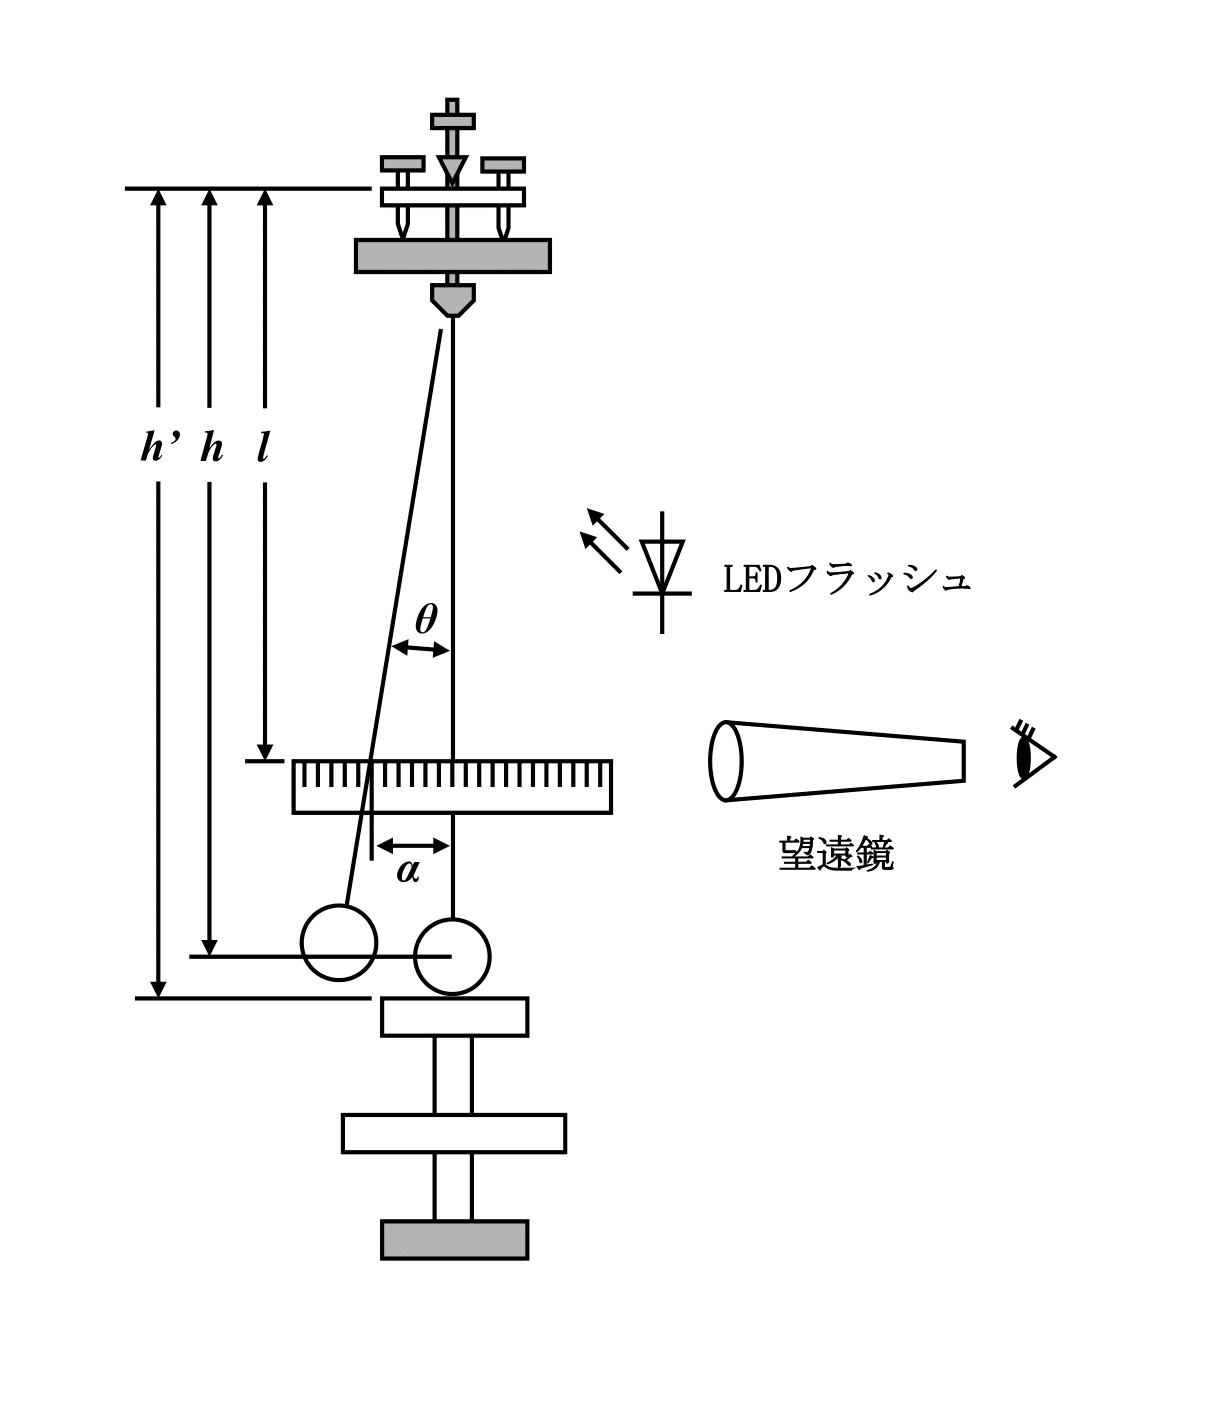
\includegraphics[width=60mm]{experimental_method_picture.png}
  \caption{振り子の実験装置}
  \end{center}
\end{figure}

正確に2秒ごとに発光するLEDフラッシュランプの光パルス(時間間隔の不確かさは$1$\textmu s以内, 発光時間は約$10$\textmu s)で振り子を照射する.
光パルスに照らされて光るピアノ線を望遠鏡で観察し, 白く光るピアノ線が左右に往復する周期$\tau$を測定する.


\section{実験結果}

\begin{table}[h]
  \centering
  \begin{minipage}{0.3\textwidth}
    \caption{$h'=1049.9\,\mathrm{mm}$}
    \begin{tabular}{cc}
        \hline
        回数 & 周期$\tau/\mathrm{s}$ \\
        \hline
        1 & 92.60 \\
        2 & 91.80 \\
        3 & 92.81 \\
        \hline
    \end{tabular}
  \end{minipage}
  \begin{minipage}{0.3\textwidth}
    \caption{$h'=1039.4\,\mathrm{mm}$}
    \begin{tabular}{cc}
        \hline
        回数 & 周期$\tau/\mathrm{s}$ \\
        \hline
        1 & 122.20 \\
        2 & 124.01 \\
        3 & 121.96 \\
        \hline
    \end{tabular}
  \end{minipage}
  \begin{minipage}{0.3\textwidth}
    \caption{$h'=1029.2\,\mathrm{mm}$}
    \begin{tabular}{cc}
        \hline
        回数 & 周期$\tau/\mathrm{s}$ \\
        \hline
        1 & 244.17 \\
        2 & 241.98 \\
        3 & 243.89 \\
        \hline
    \end{tabular}
  \end{minipage}
\end{table}

\section{考察}

\end{document}